
\chapter{Introduction}

\setcounter{chapter}{1}

Like all living organisms, the fruit fly uses sensory information
to navigate its world. To a first approximation a fruit fly's behaviour
in response to a sensory input can be described as a decision making
process of approach or retreat. One such sense that the fly uses to
decide whether to approach or retreat is the sense of smell, which
is a well-studied function, employed to gather information about the
environment, find food, mating partners, and detect dangerous conditions
signaled by harmful odours. Flies are attracted and repelled to many
odours innately (\citealp{Niewalda:2008bm}), but also show ability
to learn new odours (\citealp{Waddell:2010iw}). 

When exposed to most odours, the response behaviour of flies depends
on experience: if an odour is associated with a sweetened reward (CS+,
or conditioned stimulus) and another odour offers no reward (CS- or
unconditioned stimulus) the flies will show a preference for the rewarded
odour in a binary choice test ($Fig.\,1.1\,A$ top panel). However,
if an odour is associated with a punishment (CS+) such as a shock,
fruit flies can be conditioned aversively to odours (\citealp{Perisse:2013fpa})
and will choose the neutral odour (CS-, $Fig.\thinspace1.1\,A$ bottom
panel). Understanding how these memories of odours are generated and
how they affect behaviour is an area of current research. Researchers
are also beginning to understand how innate and learned olfactory
behaviours interact with each other. However, until now there have
been few computational driven approaches (\citealp{Luo:2010fb,Wessnitzer:2011dj})
that have converted word models into mechanistic models that can explain
mathematically the growing behavioural data, make predictions and
testable hypotheses. We shell discuss these computational methods
in Section 1.5.

\selectlanguage{british}%
\begin{figure}[H]
\selectlanguage{english}%
\includegraphics[scale=0.6]{chapter1/Figure1_circuit_a4_vers2}

\selectlanguage{british}%
\caption[The olfactory reinforcement learning circuit and experiment]{\selectlanguage{english}%
Reinforcement learning experiment and circuit \selectlanguage{english}%
}


\selectlanguage{english}%
A) In the learning paradigm the fly is shown a simple odour which
is called the CS- (conditional stimulus without reinforcement) for
2 minutes in the appetitive training protocol. Afterwards, a fly is
put into an empty chamber for 30 second where only air is present.
Finally, an odour is shown that is paired with a reinforcement (CS+)
which can be either sugar or shock. After that, the fly is tested
for odour preference when given a choice between the CS+ and CS-.
Note: In the case of aversive training, the reinforced odour (CS+)
is shown first. 

B) Normalized calcium imaging response in the $M4\beta'$ before and
after learning shows a bidirectional change in firing rate with the
calcium response increasing for aversive learning and decreasing after
appetitive learning (averaged from ten flies).

C) (i) DA neurons representing aversive reinforcement. Studies suggest
that neurons in PPL1 convey negative reinforcement and are strongly
activated by shock (\citealp{Perisse:2013fpa}). In this illustration
a selection of DA neurons innervating MB zones and the MB-M3 neurons
on the tip of the $\gamma$ lobe are activated (red). (ii) DA neurons
representing appetitive reinforcement. DA neurons in PAM innervate
many discrete zones in the $\beta$, $\beta'$ and $\gamma$ lobes.
Ca2+ imaging of sugar-evoked activity suggests only some zones receive
appetitive reinforcement. Reproduced from \citet{Waddell:2013fu}

D) The valence learning olfactory circuit is made of a group of approximately
2.000 KCs which are tasked with odour identification. There are two
groups of dopaminergic neurons that signal either shock or sugar and
depress connections between KCs and MBONs. M4 MBON biases towards
retreat behaviour while MVP2 MBONs biases towards approach behaviour.
The MVP2 MBON in this figure is show inhibiting the M4 retreat neuron
(David Owald - personal correspondence). The DPM neuron decreases
its activity during hunger and disinhibits KCs which are known to
innervate the MVP2 Approach neuron. \selectlanguage{english}%
\end{figure}


\selectlanguage{english}%

\section{Odour representation become concentration invariant in the early
stages of olfactory processes }

Flies detect odours using approximately 1,200 olfactory receptor neurons
(ORNs) housed in their antennae. The tuning of each ORN is determined
by a single odorant receptor gene, which controls whether the ORN
is broadly or narrowly tuned to odours (\citealp{Hallem:2006iu}).
Axons from the ORN expressing the same receptor always converge on
the same glomerulus. Their activity is picked up by inhibitory and
excitatory projection neurons which perform normalization of the odour
(\citealp{Luo:2010fb}). Excitatory projection neurons deliver information
to the calyces in the mushroom body while both inhibitory projection
neurons and ePNs send information to the Lateral Horn. The Lateral
Horn is associated with innate behavioral responses to odors, such
as sex-specific responses to pheromones during courtship (Datta et
al 2008), whereas the mushroom body is required for learned responses
to odors (\citealp{deBelle:1994iu}).


\section{The MB is the centre for associative learning in the fruit fly}

The mushroom bodies are symmetrical structures with each mushroom
body being composed of approximately 2,000 Kenyon Cells (\citealp{Turner:2008eo}).
Lesion experiments and synaptic blocking of mushroom bodies output
have shown that that the mushroom body plays a critical role in memory
formation and retrieval (\citealp{Heisenberg:2009bu}). While odour
coding in the antennae was dense, the MB is believed to maintain a
sparse and high-dimensional odour representation. Experimental studies
have shown that the MB maintains a sparse representation of odours
as each odour activates approximately 10\% of KCs (approximately 150
- 200 neurons , \citealp{Honegger:2011ja}). 


\subsection{Similar odours have overlapping representations in the MB}

Previous experimental studies have shown that odours with similar
chemical properties have overlapping representations in the MBs (\citealp{Campbell:2013fb}).
Behavioural experiments have shown flies have the ability to both
generalize similar odours and separate them depending on the training
protocol. If we use an odour as a CS+ and train the fly to remember
it as predicting reward the fly will showcase the same behaviour when
exposed to a previously unexposed similar odour. However if the second
odour is shown to the fly during training as the neutral odour (CS-),
the fly will not show preference to it when compared to another neutral
odour (\citealp{Campbell:2013fb}). The fly appears to be able to
be caable to both generalize similar odours and distinguish them depending
on past experience.


\subsection{The MB recurrent activity is critical for stabilizing odour memories}

Experimental studies have shown that olfactory representations in
the mushroom bodies are modulated by the anterior paired lateral (APL)
neuron (\citealp{Lin:2014io}). Each mushroom body is innervated by
a single ``giant'' APL neuron, which transmits inhibition to the
mushroom body calyx as well as the vertical and medial lobes. It also
appears that the APL receives input from KCs in the vertical and medial
lobe and inhibits KCs at their dendritic terminals in the calyx. The
APL releases GABA at a rate proportional to its level of depolarization
and appears to play a role normalizing KC responses to odours and
maintaining sparseness (\citealp{Lin:2014io}). 




\subsection{Anatomical subdivisions of the MB have unique role in odour processing }

The dendrites of the KCs form the calyx of the MB, and their axons
project anteriorly to form the peduncle before those axons terminate
in one or more lobes, termed $\alpha\beta$ $\alpha',\beta'$, and
$\gamma$ lobe ($Fig.1.2$, \citealp{Krashes:2007fh}). The $\alpha\beta$
contains 1000 KCs while the $\alpha',\beta'$ contains 600 and the
$\gamma$ lobe 400 of KCs and each subdivision is believed to have
unique roles in memory processing.

In a previous study it has been shown by blocking different anatomical
subdivisions of KCs, that the $\alpha\beta$ neurons are needed during
retrieval of aversive and appetitive memory whereas $\alpha'\beta'$
core neurons, when blocked only affect appetitive memory (\citealp{Perisse:2013fp}). 

\selectlanguage{british}%
\begin{figure}[H]
\selectlanguage{english}%
i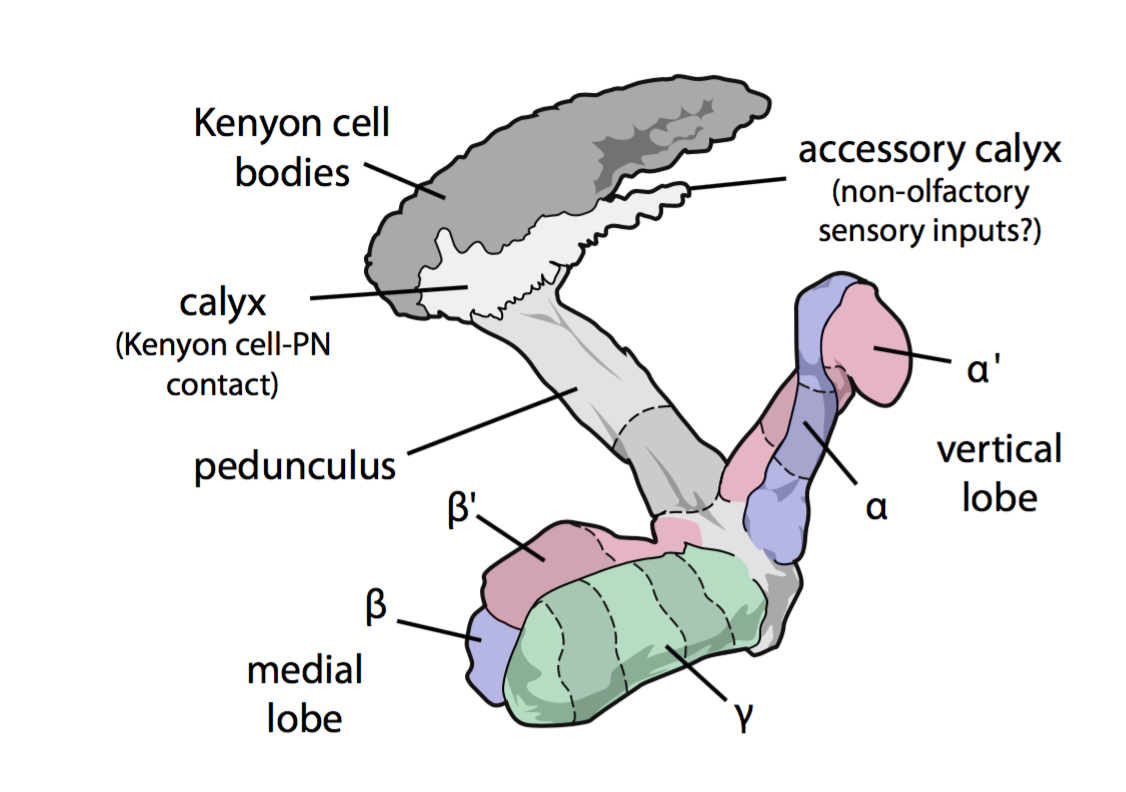
\includegraphics[scale=0.25]{chapter1/mb_divisions}

\selectlanguage{british}%
\caption[Anatomy of the Mushroom BodyAnatomy of the Mushroom Body]{\selectlanguage{english}%
 \selectlanguage{english}%
}


\selectlanguage{english}%
Gross anatomy of the mushroom body (reproduced from \citealp{Aso:2014bh}).
Dashed lines reflect the compartments defined by MBON dendrites. The
$\alpha$ and $\gamma$ lobes are each divided into three compartments,
and $\beta$ and $\beta'$ are each divided into two, $\gamma$ is
divided into five compartments.\selectlanguage{english}%
\end{figure}


\selectlanguage{english}%

\subsection{MBONs guide approach and retreat behaviours}

Outputs from approximately 2,000 Kenyon cells of the mushroom body
converge onto a population of 34 mushroom body output neurons (MBONs).
The MBON dendrites divide the two lobes and the base of the pedunculus
into a small number nonoverlapping compartments, within which the
dendrite densely contacts either all KCs or an anatomically distinct
subpopulation. KC axons in the $\alpha$/$\alpha'$ lobes are clustered
into anterior, middle, and posterior groups, in the$\beta$/$\beta'$
lobes into posterior, surface, and core groups, and in the $\gamma$
lobe into main and dorsal groups. The MBONs innervating each compartment
are genetically distinct, and each projects characteristically to
other regions of the brain. MBONs project from the mushroom body to
several regions. A small number of excitatory neurons innervating
the $\alpha$ or $\alpha'$ lobes project to lateral horn, a region
implicated in control of innate odor- related behaviors.

Every MBON projects to four neuropils just outside the mushroom body:
the crepine, the superior medial protocerebrum (SMP) the superior
intermediate protocerebrum and the superior lateral protocerebrum
where input from the approach and retreat MBONs is believed to be
transformed into motor control. 

We can classify MBONs according to the behaviour they bias towards,
as two recent studies have shown by silencing and activating each
of the 34 MBONs; they either promote approach or retreat behaviour
(\citealp{Aso:2014bh,Owald:2015cn}).

For example, experiments for one retreat promoting MBON ($M4\beta')$
have shown bi-directional change in firing rate of the neuron controlled
by the reinforcement used (appetitive or aversive). Calcium imaging
before and after training have shown the response decreases compared
to the naive response after appetitive learning and increased after
aversive learning ($Fig.2B$). Furthermore, optogenetic activation
of the $M4\beta'$ neurons changed a neutral behaviour into avoidance
behaviour and blocking the neuron converted a naive odour approach
into odour retreat in na�ve flies (flies that had an innate repulsion
to the odour without learning,\citealp{Owald:2015cn}). Converseley,
the MVP2 MBON neuron is known to promote approach behaviour. Interestingly,
there is evidence that the $MVP2$ ``approach'' MBON inhibits the
$M4\beta'$ retreat MBON ($Fig1.1D$, David Owald - private correspondence).
It is not know whether any of the retreat MBONs inhibit approach MBONs.
All though there are 32 MBONs, for our initial study we shall restrict
our modelling efforts to only two that have been studied by our experimental
collaborator: the $MVP2$ ``approach'' biasing neuron and the $M4\beta'$
retreat biasing neuron. Modelling these two neurons will allow us
to reproduce the valence coding space.


\section{DAs convey reward and punishment signals}

Dopaminergic neurons (DAs) are the most prevalent modulatory neurons
that innervate the mushroom bodies. There are distinct dopaminergic
neurons that provide positive and negative value signals. The two
major clusters where most DAs reside are the PPL and the PAM clusters
($Fig.1.1C$). Positive reinforcement are provided by subsets of the
approximately 100 DAs in the PAM cluster (\citealp{Burke:2012jt}).
They predominately innervate nearby zones in the $\beta,\beta',\gamma$
lobes. Negative reinforcement such as from electric shock or bitter
substances appears to be conveyed by DAs housed in the PPL cluster.
Each PPL DA that innervates the mushroom bodies projects presynaptic
terminals on the $\alpha$ or $\alpha\lyxmathsym{\textquoteright}$
lobe(David Owald \& Scott Waddell \textendash{} in review). The dendrites
of MBONs is restricted to few DA zones. For example for the ``retreat''
MBON we previously discussed ($M4\beta'$ ) experimental data exists
to support that the axons from sugar rewarding dopaminergic neurons
overlap with the dendrites of the MBON (\citealp{Owald:2015cn}).


\subsection{DAs convey reward and punishment signals in different areas of the
mushroom body }

Distinct DAs convey the effects of sugar and water reward as opposed
to the same neurons representing subjective value such as in the case
of negative reinforcing DAs (\citealp{Perisse:2013fp}). The sugar
and water responsive DAs project to unique zones on the MB lobes,
thus suggesting that learning-related plasticity is represented at
different axon terminals along the lobes of the mushroom body. It
is believed that since DAs reaches a subset of KCs axons, they modify
KC output synapses onto MBONs in their respective zone. Thus water
memories and sugar memories are predicted to have unique KC-MBON connections
that represent them (\citealp{Lin:2014ix}).


\subsection{DA state control}

Sugar memory is most robustly expressed in hungry flies and similarly,
thirst promotes the expression of water memory. It appears that to
form these memories, different zones of the MB provides the anatomical
requirements in which state control be implemented. Interestingly,
a group of DA neurons that provide the inhibitory constraint to the
expression of sugar memory (\citealp{Lin:2014ix}) occupy the same
zones in the heel and peduncle of MB as the MVP2 approach neuron whose
activity drives approach behaviour. Thus it seems likely that the
internal state of hunger skews the balance of MBON pathways to favour
approach. It has not been yet shown whether the activation of thirst
involves a similar layer of control. A current study has shown that
the MVP2 ``approach'' neuron increases its response to an odour
after it has been starved which biases the behaviour towards approach
(David Owald - personal correspondence, $Fig\,.\,1.3$). This adds
another layer of complexity to the valence learning model which is
state modulation of behaviour.

\selectlanguage{british}%
\begin{figure}[H]
\selectlanguage{english}%
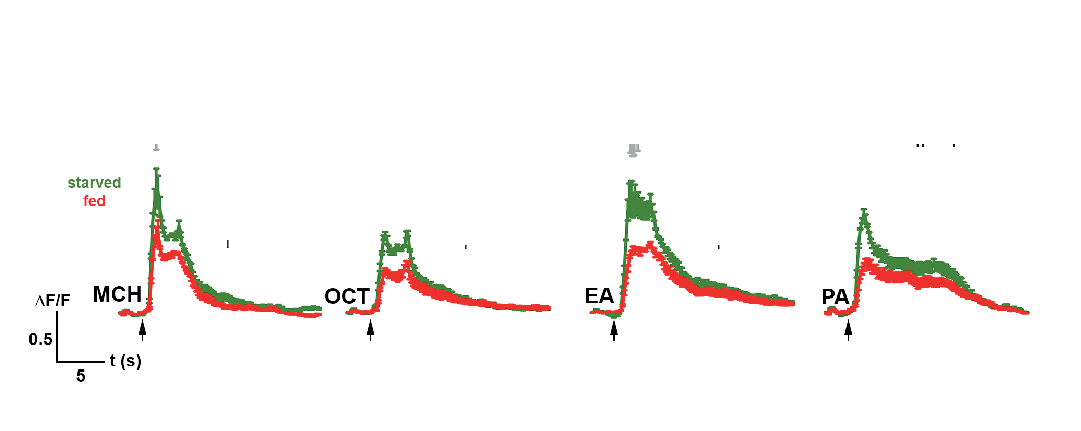
\includegraphics[scale=0.2]{chapter1/Fig_starved_vs_fed}

\selectlanguage{british}%
\caption[Activity in the MVP2 neuron starved and fed]{\selectlanguage{english}%
 Normalized calcium imaging response of the MVP2 neuron to four different
odours, averaged from ten flies. \selectlanguage{english}%
}
\end{figure}


\selectlanguage{english}%

\subsection{DA modulated learning changes odour drive to KC-MBON synapses}

A hypothesis of how valence learning is achieved, proposes that learning
modifies subsets of KC-MBON pathways which in naive flies are balanced
(\citealp{Owald:2015cn}). Appetitive responding DAs promote odor
approach by depressing odor drive to ``avoidance'' MBONs and possibly
by strenghtening approach pathways. Conversely, aversive responding
DAs promote depressing odour drive to ``approach'' MBONs \citep{Aso:2014bh}.
It is likely that a feedack loop from MBON to DAs influences learning
as well. Blocking the $M4\beta'$ neuron induced a depression of the
KC-$M4\beta'$ MBON connection (\citealp{Owald:2015cn}), which could
be because the $M4\beta'$inhibits some appetitive DAs. 


\section{Spike Timing Dependent Plasticity (STDP) as a candidate for plasticity
at the KC-MBON synapses}

A candidate mechanism for valence learning has been proposed in a
recent study in the locust, a similar system to Drosophila (Cassenaer
and Laurent 2012). They have shown that KC-MBON synapses usually obbey
the spike-timing-dependent plasticity (STDP) rule. STDP can be seen
as a spike-based variant of the Hebbian rule where synaptic change
depends on the relative timing of pre and postsynaptic action potential
(\citealp{Bi:1998ve}). During STDP, a synapse potentiates when the
postsynaptic spike happens after the pre-synaptic spike within a time
window of the order of tens of milliseconds and depresses when the
order is reversed (\citealp{Bi:1998ve}). Spike timing, however is
not sufficient to explain how plasticity strengthens or weakens synapses.
Neuromodulators such as dopamine can gate plasticity determining when
learning can take place (\citet{Pawlak:2010cn}). Indeed, in the locust
when octopamine was injected 1 s after spike pairing in the experimental
protocol synapses were only observed to depress their strength ($Fig.2.1B$).
In flies octopamine is known to act on the mushroom body indirectly,
by activating PAM dopaminergic neurons (\citealp{Waddell:2013fu}).
Therefore evidence from studying the locust supports the hypotheses
of dopamine modulated STDP as the candidate mechanism for learning
in the fruit fly. 


\section{Previous modelling attempts of olfactory learning}

Previous modelling efforts of the fruit fly's olfactory circuit have
mostly focused on the neurons implicated in olfactory processing before
reaching the MBONs, since 3 landmark papers this year opened the path
to modelling them \citep{Hige:2015er,Owald:2015cn}, \citealp{Aso:2014bh}).

However, there has been one study that reproduced the valence learning
capacity of the olfactory circuit (\citealp{Wessnitzer:2011dj}).
They created a spiking model with dopamine modulated plasticity occurring
at the synapses between KCs and MBONs and have show that the MBON
can learn to distinguish between odours of opposite valences. In their
model, contrary to current evidence dopamine potentiates the weights.
Their model predicts the fly can also learn an odour mixture discrimination
task where one half of the odour is paired with a negative reinforcement
and another half is neutral which has been shown experimentally in
the bee (\citealp{Giurfa:2003dd}). 


\section{Improving previous models of valence learning in the fruit fly}

The model that was previously discussed (\citealp{Wessnitzer:2011dj})
have provided us with a good starting point, since it implemented
a dopamine modulated learning rule that allows the model to classify
odours of different valences witth a single MBON. However, we modelled
two type of MBONs, which allows us to visualize the coding space for
``retreat'' and ``approach'' behaviours. Furthermore we have also
studied competition between MBONs which code for opposite valences.
Finally, we have studied for the first time in the fruit fly the functional
consequences of bi-directional change of firing rate in MBONs. 


\chapter{Methods}

Experiments of the $M4\beta'$ and $MVP2$ MBONs were performed by
David Owald at the CNCB and motivated the simulations which were created
by the author. We decribe the first stage of our modelling efforts
where we tested a plasticity learning rule that depresses the synapse
in the presence of dopamine. The three main neuron types that we modelled
heere are Kenyon Cells, MBONs and DAs.


\section{Connectivity}

We used experimental data that traces the connectivity between KCs
and output neurons (\citealp{Aso:2014bh}). The $M4\beta'$ neuron
receives input from 500 KCs from the $\alpha'\beta'$ lobe and 400
KCs from the $\alpha\beta$ lobe. The MVP2 neuron receives input from
400 KCs from the $\gamma$ lobe and 500 KCs from the $\alpha'\beta'$
lobe. We do not know the initial synaptic efficacies (weights) between
KCs and MBONs, thus we make the assumption that the weights between
KCs and MBONs have uniform random strengths at start. By doing that
we found that we needed to tune our synapses with strengths between
0 nS and 2 Ns to achieve MBON firing rates of 50 Hz, whic is in accordance
with experimental evidence \citep{Hige:2015er}. 


\section{MB Kenyon Cells model}

When the fly is exposed to an odour \textasciitilde{}200 KCs activate.
The two MBONs sample approximately half of the total number of KCs,
thus only a hundred odour responding KCs send an input MBON. We modelled
the spike trains for 100 KCs in response to an odour based on experimental
data (\citealp{Turner:2008eo}). In our model an odour is represented
as KC spikes. In our protocol we first select 100 KCs that will be
active to an odour and send input to each MBON. 

During spontaneous activity each KC fires at approximately \textasciitilde{}0.1
Hz. Whole cell recording have shown that when an odour is shown KCs
fire an average of 3 spikes per second. In normalized calcium imaging
experiments, KCs are found to show a larger response in the first
200 ms of the odour exposure (\citealp{Turner:2008eo}). We have used
this information to generate KC spike trains with an average of 3
spikes per second and with a higher probability of a spike to occurr
in the first 200 ms compared to the rest of time.  


\section{MBONs model}

As a starting point we have modelled two MBONs, one for approach and
one for retreat ($M4\beta'$  and $MVP2$). As previously discussed,
each MBON samples half of the total number of KCs. The firing rate
of the ``approach'' $MVP2$ neuron is determined entirely by input
KCs. For each simulatuion the $M4\beta'$ neuron receives inhibition
from the $MVP2$ MBON, which is accordance with experimental evidence
( David Owald - unpublished work). We used a Linear Integrate and
Fire (LIF) model with parameters that were taken from a recent modelling
paper where whole cell recordings of MBONs was performed \citep{Hige:2015er}.

\begin{table}[h]
\begin{tabular}{ccc}
\hline 
\multicolumn{1}{c}{Parameter} & \multicolumn{1}{c}{Default Value} & \multicolumn{1}{c}{Symbol }\tabularnewline
\hline 
 &  & \tabularnewline
\hline 
MBON Membrane Time Constant  & 20 ms  & $\tau_{m}$\tabularnewline
\hline 
MBON Spiking threshold  & -40 mV  & $V_{th}$\tabularnewline
\hline 
MBON Resting membrane potential  & -60 mV  & $V_{inh}$\tabularnewline
\hline 
MBON Excitatory conductance  & 0 mV  & $E_{ex}$\tabularnewline
\hline 
MBON Inhibitory conductance  & -80 mV  & $E_{inh}$\tabularnewline
\hline 
\end{tabular}

\caption{MBON neuron parameters}
\end{table}



\section{LIF Neuron Model}

We used the conductance based LIF model to model the MBONs. The LIF
neuron equation is as follows:

\begin{equation}
\tau_{m}\frac{dV}{dt}=(V_{rest}-V(t))+g_{ex}(E_{ex}-V(t))+g_{inh}(E_{inh}-V(t)).
\end{equation}
\begin{minipage}[t]{1\columnwidth}%
Here V is the membrane potential of the neuron as a function of time
, $\tau_{m}$is the membrane time constant, $V_{rest}$is the resting
membrane potential, $E_{ex}$is the excitatory reversal potential
and $E_{in}$is the inhibitory reversal potential. The synaptic conductances
are expressed by $g_{ex}$(excitatory) and $g_{inh}$(inhibitory).
They are modelled according to the following equations:%
\end{minipage}

\begin{equation}
\tau_{ex}\frac{dg_{ex}(t)}{dt}=-g_{ex}(t)
\end{equation}
\begin{minipage}[t]{1\columnwidth}%
and%
\end{minipage}

\begin{equation}
\tau_{inh}\frac{dg_{inh}(t)}{dt}=-g_{inh}(t),
\end{equation}


where $\tau_{ex}$and $\tau_{inh}$are the synaptic time constants
for the excitatory and the inhibitory conductance, respectively. When
the neuron receives an action potential from a presynaptic cell the
postsynaptic conductance increases by the following formulas: $g_{ex}\rightarrow g_{ex}+\Delta g_{ex}$
and $g_{inh}\rightarrow g_{inh}+\Delta g_{inh}$ for excitatory and
inhibitory synapses, respectively. 


\section{The three-factor plasticity learning rule}

We introduce an STDP (Spike-Timing Dependent Plasticity) learning
rule into our model has been observed in the locust mushroom bodies
(\citealp{Cassenaer:2007go}). In this dopamine modulated STDP model, 

Synaptic change in our model is the result of dopamine concentration
value multiplied by synaptic tag value at each time point.

Synaptic weight change is gated by the presence of dopamine. Eq. 2.9
shows that weight change occurs when dopamine concentration is above
0. Change is negative according to experimental evidence so we multiply
by -1. 

\begin{equation}
\frac{\text{d}w_{ij}(t)}{\text{d}t}=D(t)c_{ij}(t)
\end{equation}


We model the DA neuron as an integrate and fire neuron which determines
the value of the final component of our learning rule. The neuron
receives direct current input in the presence of a reward or a punishment
depending on the training method use and fires regularly at a rate.
The dopamine concentraftion (D(t) which modulates synaptic change
is a global eligibility trace that increases each time the dopamine
neuron fires,

\begin{equation}
D(t)=-\frac{D(t)}{\tau_{d}}+\sum_{k}\delta(t-t_{k}^{*}),
\end{equation}
\begin{minipage}[t]{1\columnwidth}%
where $t_{k}^{*}$is the k-th DA spike and $\delta$ is the Dirac's
delta. $c_{ij}$ represents a temporal tag in synapses where pre-post
firing occurs,%
\end{minipage}

\begin{equation}
\frac{\text{d}c_{ij}(t)}{\text{d}t}=-c_{ij}(t)/\tau_{c}-A_{-}x_{j}(t)S_{i}(t)-A_{-}y_{i}(t)S_{j}(t),
\end{equation}
where $A_{-}$dtermines the amplitude of maximum depression that the
synapse can undergo when presynaptic and postsynaptic spikes times
occurr nearly at the same time. $S_{i}(t)$ is the spike train of
the i-th neuron, given by

\begin{equation}
S_{i}(t)=\sum_{k}\delta(t-t_{i,k}^{*}),
\end{equation}
\begin{minipage}[t]{1\columnwidth}%
where $t{}_{i,k}^{*}$ is the timing of the spike, where $i$ is the
i-th neuron and $k$ is the index of the spike. The tag decreases
when the postsynaptic neuron fires an action potential and depends
on the timing of the last spike timings of the presynaptic neuron
through the variable $x_{ij}(t)$ which evolves accordingly to: %
\end{minipage}

\begin{equation}
\frac{dx_{j}(t)}{dt}=-\frac{x_{j}(t)}{\tau_{-}}+S_{j}(t).
\end{equation}
\begin{minipage}[t]{1\columnwidth}%
Equally the tag also decreases when the presynaptic neuron fires an
action potential, depending on the postsynaptic neuron activity through
the variable $y_{ij}(t)$ given by%
\end{minipage}

\begin{equation}
\frac{dy_{i}(t)}{dt}=-\frac{y_{i}(t)}{\tau_{-}}+S_{i}(t),
\end{equation}
\begin{minipage}[t]{1\columnwidth}%
where $\tau_{-}$ is the characteristic time of the $y_{i}$ and $x_{i}$eligibility
traces. %
\end{minipage}

\begin{figure}[h]
\hfill{}Table 2\hfill{}

\hfill{}%
\begin{tabular}{ccc}
\hline 
\multicolumn{1}{c}{Parameter} & \multicolumn{1}{c}{Default Value} & \multicolumn{1}{c}{Symbol }\tabularnewline
\hline 
 &  & \tabularnewline
\hline 
STDP max Depression amplitude  & 0.005  & $A_{-}$\tabularnewline
\hline 
STDP Depression time constant  & 20 ms  & $\tau_{-}$\tabularnewline
\hline 
Dopamine time constant & 20 ms & $\tau_{d}$\tabularnewline
\hline 
\end{tabular}\hfill{}
\end{figure}


The STDP parameters we used were previously measured experimentally
in vivo in the STDP learning paradigm (\citealp{Abbott:2000gg}).
In our learning paradigm dopamine gates synaptic learning which is
to say synaptic change can not occurr in the absence of dopamine.
We have used a general model of dopamine gated STDP learning (\citealp{Izhikevich:2004ul}). 

\selectlanguage{british}%
\begin{figure}[H]
\selectlanguage{english}%
\includegraphics[scale=0.7]{chapter1/Figure3_learningrule}\foreignlanguage{british}{\caption[Learning components at the KC-MBON synapse]{\selectlanguage{english}%
Learning components at the KC-MBON synapse\selectlanguage{english}%
}
}

\begin{minipage}[t]{1\columnwidth}%
A) KC-MBON STDP learning rule, reproduced from Cassenaer and Laurent
(\citealp{Cassenaer:2007go}). In gray, the normal STDP rule in KC-MBON
synapses, where $\delta$t is the time of the postsynaptic spike minus
the presynaptic spike, and the y axis shows the percent change in
KC-evoked EPSP size in MBONs following five trials in which pre- and
postsynaptic spikes were paired at the given $\delta$t. In blue,
the STDP rule observed when octopamine is injected 1s after pairing.
B) Dopamine modulated spike-timing dependent learning rule: Near-coincident
pre- and postsynaptic spikes induces synaptic depression. C) i) Raster
plot showing KCs firing in response to an odour ii) $M4\beta'$  neuron
membrane potential during appetitive training iii) Excitatory (green)
and Inhibitory (currents) during appetitive training D) i) The relative
timing of firings of the pre and post synaptic neurons induce changes
in the synaptic 'tag' variable according to the dopamine modulated
STDP learning rule. ii) The synaptic tag decays to zero (top), but
if extracellular dopamine are present during the critical time window
(middle) the maximal synaptic conductance w is modified (iii) The
synaptic weight, here written as w depresses as there have been pre-post
spike pairs and dopamine is present in the system%
\end{minipage}\selectlanguage{english}%
\end{figure}


\selectlanguage{english}%

\section{Odour exposure protocol}

In our learning paradigm we require KCs and MBONs to spike, together
with the presence of dopamine. Whole cell recordings have shown how
KCs respond when exposed to an odour over 1 second, firing at approximately
3 Hz, compared to a spontaneous activity of approximately 0.1 Hz (\citealp{Turner:2008eo}).
We can not know if the KCs fire constantly at 3 Hz for the entire
duration of appetitive or aversive conditioning or whether they adapt
to the odour and return to spotaneous activity. It is however sufficient
to show an odour for 2 seconds coincident with reward or punishment
for learning to take place (Johannes Freisenbrug - personal correspondence).
For this reason we showed the odour for 2 seconds in our training
paradigm. 


\chapter{Results}

Our experimental collaborator has shown that when calcium imaging
the $M4\beta'$ neuron, the activity changed both after appetitive
and after aversive training. The $MVP2$ MBON is known to change its
firing rate only after aversive training. We simulated the $M4\beta'$
and the $MVP2$ MBONs during these two scenarios to check the prediction
$(\mbox{Fig\,.\,3.2}$) and visualized the coding space the two MBONs
form ($Fig$.~3.1).


\section{Odours have a balance of approach and retreat drive before training}

In our model the firing rate of the3 $M4\beta'$  neuron determines
the retreat drive of an odour, while the firing rate of the $MVP2$
MBON determines the drive to approach. We visualized the valence coding
space by plotting their firing rates on two different axes ($Fig.\,3.1$).
Using our protocol we generated two different odours by creating stereotypical
KC responses. MBONs had a balanced drive of approach and retreat before
training, which is to say the firing rate of the $M4\beta'$  and
$MVP2$ neurons are approximately equal ($Fig.3.1$). Training an
odour with appetitive reinforcement decreased their drive towards
retreat while, training with aversive reinforcement both decreased
their drive towards approach and increased their retreat drive.

\selectlanguage{british}%
\begin{figure}[H]
\selectlanguage{english}%
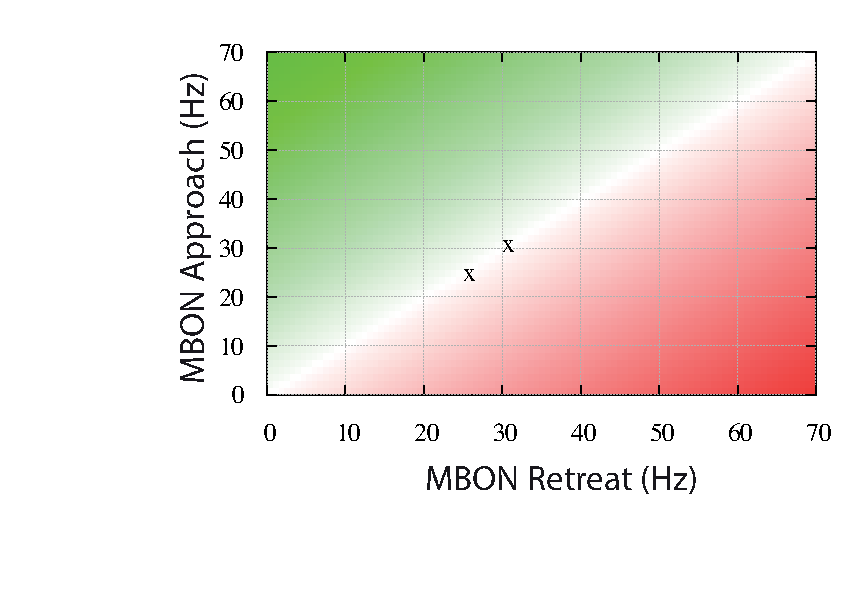
\includegraphics[scale=0.65]{chapter1/odor_space2}

\selectlanguage{british}%
\caption[MBON coding space before learning]{\selectlanguage{english}%
MBON coding space before learning \selectlanguage{english}%
}


\selectlanguage{english}%
This figure shows the odor valence space coded by MBONs. The white
line represents a perfect balance between retreat and approach drive
corresponding to both MBONs populations firing at the same rate. The
green area corresponds to a higher drive towards approach. Conversely,
the red area corresponds to a higher retreat drive from MBONs. \selectlanguage{english}%
\end{figure}


\selectlanguage{english}%

\section{Bi-directional change in firing rate can occur when dopamine depresses
the KC-MBON synapses}

We simulated an appetitive and aversive training protocols by showing
odours for 2 seconds. In the presence of dopamine. We monitored the
plasticity was active at the KCs-MBONs synapses and how this affected
odour response before and after learning. 

We observed that during appetitive training KC-$M4\beta'$  synaptic
weights decreased ($Fig.\,3.2\,A,$ ii). After learning, the response
from the $M4\beta'$  neuron shows a decreased firing rate profile
compared to the naive state ($Fig.\,3.2\,A$ iii). The firing rate
decreased by 5 Hz compared to the initial state. Conversely, aversive
learning increased the response of the $M4\beta'$  neuron compared
to the naive state ($Fig.\,3.2\,B$ iii). This is due to the fact
that the firing rate of the MPV2 neuron decreased ($Fig.\,3.2\,B\,iv$),
thus increasing the ratio of excitation to inhibition ($Fig\,.3.3$).

To observe a change in the firing rate that qualitatively matched
the experimental results ($Fig\,1.2\,B)$ wee had to choose the strength
of the inhibitory MVP2-$M4\beta'$ synapse that increased the ratio
of excitation to inhibition ($Fig.\,3.4)$. The MBONs we modelled
receive input from 100 KCs which fire at a rate of 3 Hz. Every second
they receive 300 excitatory spikes with an average weight of 1 nS.
In comparison the $M4\beta'$  inhibiting MVP2 neuron fires at a rate
of approximately 50 Hz. To obtain the increase in firing rate that
qualitatively matches experimental results ($Fig\,1.2\,B)$ we had
to tune the weight of the inhibitory synapse to be twice as strong
at the excitatory synapse. 

The odour representation in valence space moves perpendicularly to
the line of equal drive and thus has a strong affect, whereas appetitive
training moves along a single axis. This can be explained due to the
fact that aversive learning both decreases drive to the approach MBON
and increase drive to the retreat MBON. 

\selectlanguage{british}%
\begin{figure}[H]
\selectlanguage{english}%
\includegraphics[scale=0.7]{chapter1/Figures3_clean2}\foreignlanguage{british}{\caption[text to list of figures]{\selectlanguage{english}%
 Responses of the MVP2 (approach) and$M4\beta'$(retreat) neurons\selectlanguage{english}%
}
}

A) During appetitive training the dopamine modulated STDP rule targets
the KC-$M4\beta'$  synapses i) In our simulation an odour is shown
for 1 s while appetitive reinforcement is provided after 100 ms ii)
A selection of 'weights' are shown that represent the efficacy of
the KC-$M4\beta'$  synapses (blue) undergoing depression iii) Before
(black) and after appetitive learning (light blue) $M4\beta'$ response
to the odour iv) Before (black) and after (purple) appetitive learning
response of the MVP2 neuron. B) During aversive training dopamine
modulated STDP targets the KC-MVP synapse leading to disinhibition
of the M4 neuron i) An odour is shown for 3 s paired with aversive
reinforcement ii) A selection of 'weights' are shown that represent
the efficacies of KC-MVP synapses (purple). iii) Before (black) and
after aversive learning (light blue) $M4\beta'$ response to the odour
iv) Before(black) and after (purple) aversive learning response of
the MVP2 neuron.\selectlanguage{english}%
\end{figure}


\begin{figure}[H]
\selectlanguage{english}%
\includegraphics[scale=0.6]{\string"chapter1/Figure20 - before_after\string"}\foreignlanguage{british}{\caption[text to list of figures]{\selectlanguage{english}%
MBON coding space after learning \selectlanguage{english}%
}
}

A) The odour is shown before and after appetitive learning in valence
coding space which shifts its position towards the green area of the
valence space B) The odour is shown before and after aversive learning
in the valence coding space which shifts its position towards the
red area of the valence space. \selectlanguage{english}%
\end{figure}


\begin{figure}[H]
\selectlanguage{english}%
\includegraphics[scale=1.2]{chapter1/currents_before_after_aversive}\foreignlanguage{british}{\caption[text to list of figures]{\selectlanguage{english}%
\selectlanguage{english}%
}
}

A) Synaptic current of the $M4\beta'$ neuron before aversive training
B) Synaptic currents of the $M4\beta'$ neuron after aversive training\selectlanguage{english}%
\end{figure}


\selectlanguage{english}%

\section{Inhibition between MBONs can enhance odour discrimination}



To show that the MVP2-M4 inhibitory synapse is necessary and that
it enhances dsicrimination we performed the simulation in two conditions,
once with the MVP2-M4 inhibitory synapse active ($Fig.3.5A$) and
once without ($Fig.\,3.5\,B$). The M4 MBON increases its firing rate
only when there is an inhibitory synapse between the MVP2 and M4 Furthermore,
if we look at the valence coding space (Figure 9 bottom), we observe
that the inhibitory synapse between the MBON increases discriminability
by pushing the representation depeer into the reretreat area ($Fig.3.5B$
bottom). 

\selectlanguage{british}%
\begin{figure}[H]
\selectlanguage{english}
\includegraphics[scale=0.7]{chapter1/Figure7_lateral_inihibition_vers2}\foreignlanguage{british}{\caption[text to list of figures]{\selectlanguage{english}%
 Aversive learning with and without MVP2 - $M4\beta'$inhibition\selectlanguage{english}%
}
}

To see the functional implications of lateral inhibition we pair an
odour with aversive reinforcement and perform the simulation for 1
second with and without inhibition. A) Odour retrieval test without
lateral inhibition In order: i) Response of approach neuron to odour
after aversive training vs naive response ii) Response of retreat
neuron to odour after aversive training vs. naive response iii) Odour
before and after training in coding space B) Odour retrieval test
with lateral inhibition. i) Response of retreat neuron to odor after
aversive training vs. naive ii) Response of approach neuron after
aversive training vs. naive; iii) Odor projected in valence space
before and after training \selectlanguage{english}%
\end{figure}


\selectlanguage{english}%

\section{Trained odour can change the valence of a similar untrained odour }

Based on evidence that similar odour activates an overlapping subset
of KCs in the MB we tested in our mnodel how learning affects untrained
odours on our model. 

We have selected two odours with 50\% overlap in the identity of KCs
activated two mimick similar odours that appear in nature. In the
naive state, both of the odours have a neutral valence ($Fig3.6$).
We subsequently trained, the first odour with both appetitive and
aversive reinforcement. When we tested both of the two odurs for their
response in the MBON code space we observed that both odours have
changed the valence to that of the trained odour ($Fig.\,3.6$) which
has been shown experimentally to occurr (\citealp{Campbell:2013fba}). 



\selectlanguage{british}%
\begin{figure}[H]
\selectlanguage{english}%
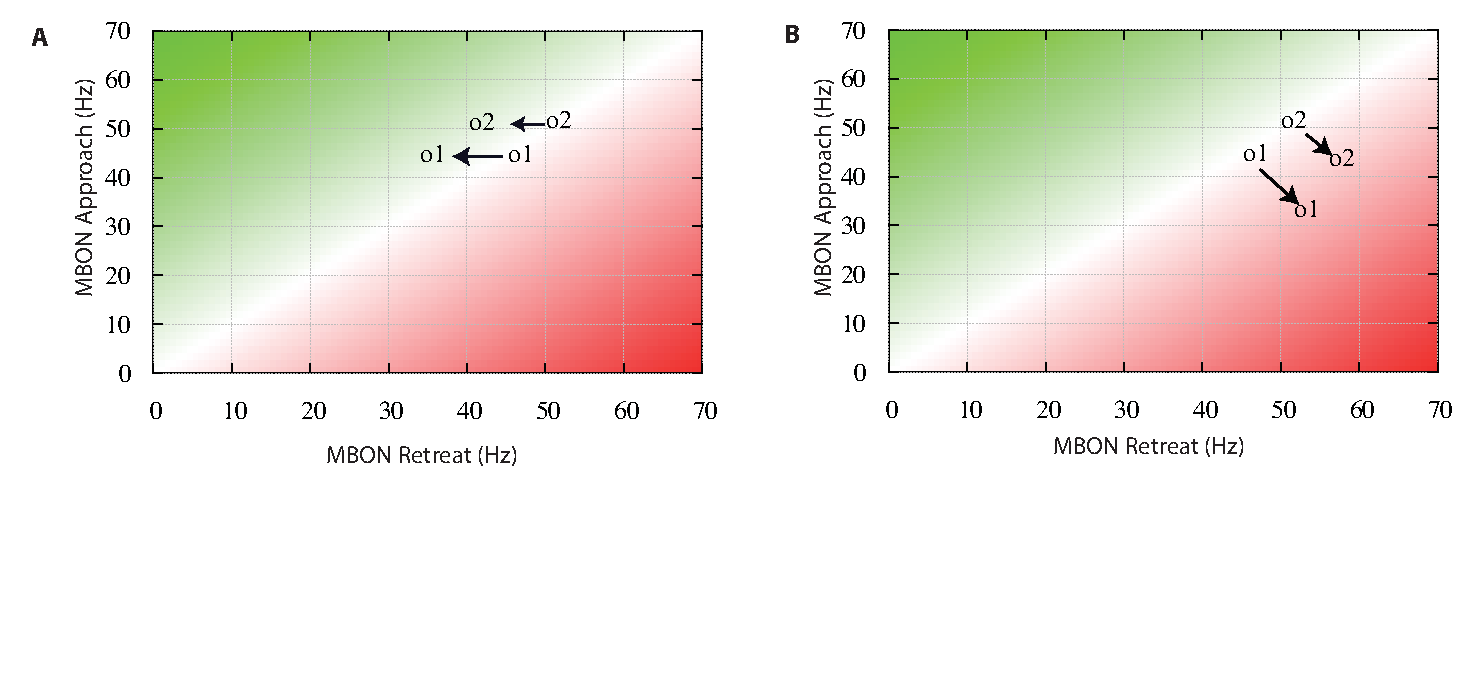
\includegraphics[scale=0.6]{chapter1/Figure7_overlap2_new.ai}\foreignlanguage{british}{\caption[text to list of figures]{\selectlanguage{english}%
Training odours with overlapping representations\selectlanguage{english}%
}
}We have trained an odour with an appetitive (A) / aversive (B) stimulus
(o1) and we visualize both the trained odour and a similar odour with
overlap after o1 is trained. A) Bot the trained (o1) odour and the
untrained (o2) have moved position in the valence space towards the
approach area B) Both the trained (o1) and the untrained (o2) odour
with overlapping representation havee moved their position in the
valence space to the aversive area\selectlanguage{english}%
\end{figure}


\selectlanguage{english}%

\section{Aversive memories are more stable than appetitive memories}

We have shown that aversive learning leads to enhanced discriminability
when compared to appetitive training in our model $(Fig\,3.4\,B$
iii). This motivated us to test the following two scenarios. We have
trained one odour with appetitive reinforcement first and aversive
training aftewards to observe the change in the position it occupies
in the odour valence space ($Fig\,3.5\,A$). Appetitive training for
2 seconds leads to a decrease in the firing rate of the M4 neuron
(retreat) and converts the neutral odour into an odour that signals
approach ($Fig\,3.5\,A)$. When we induce aversive learning immediately
afterwards, we observe a decrease in the firing rate of the MVP2 neuron
(approach) and an increase in the firing rate of the M4 neuron. The
bi-directional change of firing rate converts the odour from signaling
approach to signaling retreat. Conversely in the following simulation
we tested what happend when we chose to train the odour aversively
first. The perpendicular movement in the coding space ($Fig\,3.5\,B$)
due to bi-directional change in the firing rate ensured that the odour
remained aversive even after we induced appetitive training. In our
simulation we observed that his result depends on whether appetitive
and aversive learning decrease the firing rate of the targeted neuron
in an equal manner. 

\selectlanguage{british}%
\begin{figure}[H]
\selectlanguage{english}%
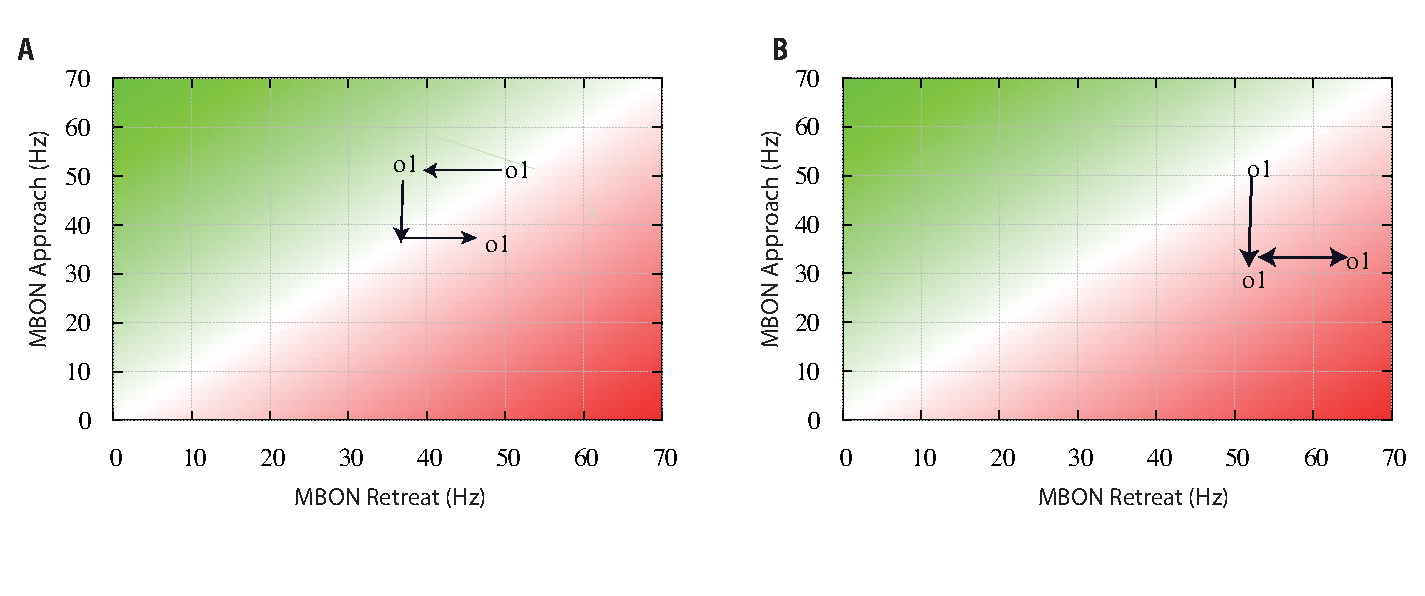
\includegraphics[scale=0.45]{chapter1/Final_figure_trained_twice.ai}\foreignlanguage{british}{\caption[text to list of figures]{\selectlanguage{english}%
 Training an odour with two types of reinforcement successively\selectlanguage{english}%
}
}

A) We have trained a single odour first with an appetitive reinforcement
and afterwards with aversive reinforcement. The odour first occupied
a position in the approach area of the MBON valence space. After aversive
training the odour moved into the area of the retreat valence space
B) We have now trained an odour with an aversive reinforcement first
and afterwards with appetitive reinforcement. The odour remained in
the retreat area of the valence space after the two types of training. \selectlanguage{english}%
\end{figure}


\selectlanguage{english}%

\chapter{Discussion and future work}


\section{Conclusions from preliminary results}

We have begun to explore how sparse odour information stored in a
balanced spiking network can be read by the MBONs through a multifactor
learning rule. We have used recent evidence that suggests that approach
MBONs inhibit retreat MBONs (David Owald - personal communication)
and have shown that MBON-to-MBON inhibition can lead to enhanced discrimination
($Fig3.4$). Enhanced discrimination is a property that is useful
for a system classifying odours, thus it could be possible that there
are retreat biasing MBONs that inhibit approach biasing MBONs. If
this is true than both aversive and appetitive learning would induce
bi-directional changes of firing rate into subsets of ``approach''
MBONs and ``retreat'' MBONs. In our model we tested bi-directional
change that occurrs only during aversive learning. In such a scenario,
we predict that training the same odour successively with both aversive
and appetitive reinforcement would change the valence from appetitive
to aversive if the odour was trained appetitive first and keep the
valence aversive if aversive training occurred first. Our results
suggest that in the fruit fly good odour memories with are easier
to convert into bad memories and bad memories are more resilient.

We have visualized the coding space created by the firing rates of
the MBONs create in response to an odour. The valence space was inspired
by experimental evidence that shows the highest degree of separation
in terms of MBON firing rates is when odours have different valances
rather than different identities (\citealp{Hige:2015er}). While MBONs
may be very good at separating odours based on their valences it could
be possible that other information could be stored in the spike times
of the MBONs, such as information about odour identity or qualitative
factors such as what kind of reward the odour predicts: water, food,
mating. It is also worth noting that the experimental paradigm uses
simple stimuli to train the fly which might restrict the ability of
the neuron to learn complex interactions. For example we know that
the flies are capable to associate an odour that predicts another
odour that predicts reward which is called second ordour conditioning
(\citet{Wu:2007ie}).


\section{Future work}


\subsection{Learning over larger periods of time}

We have modelled two dopaminergic neurons in our model one for each
learning scenario: appetitive and aversive. The dopaminergic neurons
create a temporal window in which plasticity can depress a synapse.
The time window during which coincidence spikes and dopamine presence
can depress a synapse is 20 ms in our model. However, there is evidence
that the outcome of learning depends on the timing of the odour and
the punishment over larger intervals of time (\citealp{Yarali:2008dt})
A fly that is shown an odour first and shocked 15 s later will learn
to avoid the odour (\citealp{Yarali:2008dt}). If the sequence is
reversed and a fly is shocked first the odour will become appetitive
(\citealp{Yarali:2008dt}). Further more if a fly is shocked with
a strong shock first paired with an odour and a milder shock later
paired with a different odour the fly will learn to approach the second
odour (\citealp{Perisse:2013fp}). Our model fails to replicate these
results that belongs to the paradigm of relief learning because the
shock signal always leads to depression of the approach pathway in
our model. One possible solution to this problem could be that the
activity of appetitive and aversive dopaminergic neurons is relative
to past experiences. In our model we can test a paradigm, where when
we would stop a shock signal after a period of time, the aversive
dopaminergic neurons will decrease their activity and the appetitive
dopaminergic neurons will show an increase in their activity.


\subsection{Second order conditioning}

In our first model investigating plasticity in the MB we have used
a learning rule that leads to synaptic depression when dopamine in
present (\citealp{Greenspan:2004iu}). However, the fly is able to
learn to apparoach an odour that predicts another appetitively trained
odour. This could be because during second order conditioning when
the fly is exposed to the appetitive odour, appetitive dopaminergic
neurons increase their activity which makes the fly susceptible to
learn to consider the second odour as being appetitive. We would likje
to explore how we can tune the activity of dopaminergic neurons in
response to not only reward and punishment but also stimuli that were
learned. A candidate mechanism that could explain this might be the
feedback loop from MBONs to DAs.


\subsection{Implementing the MBON - DA feedback loop}

We have begun preliminary work on investigating the MBON - DA feedback
loop. Recent anatomical work shown that the $M4\beta'$ ``retreat''
biasing MBON has axons projecting to appetitive DA neurons \citep{Owald:2015cn}.
We would like to examine the functional consequences that such a feedback
loop has to learning and test different scenarios - what happens when
the feedback loop is excitatory or inhibitory.


\subsection{State dependent memory retrieval }

Our experimental collaborator has recently shown that the approach
MVP2 output neuron increases its response to an odour when the fruit
fly is hungry ($Fig\,1.3$). This implies that the olfactory circuit
is modulated by the behavioural state of the organism. A plausible
mechanism which has been explored in cortex is inhibition, which has
been linked to brain states such as attention (Harris and Thiele 2011,
Stringer et al., 2015 ). We would like to explore how inhibition in
the MB changes in response to motivational state. A candidate neuron
mechanism might be APL state dependent inhibition, which is a neuron
that inhibits the entire population of KCs (\citealp{Lin:2014io}). 


\chapter{Timeline}

\selectlanguage{british}%
\begin{figure}[H]
\selectlanguage{english}%
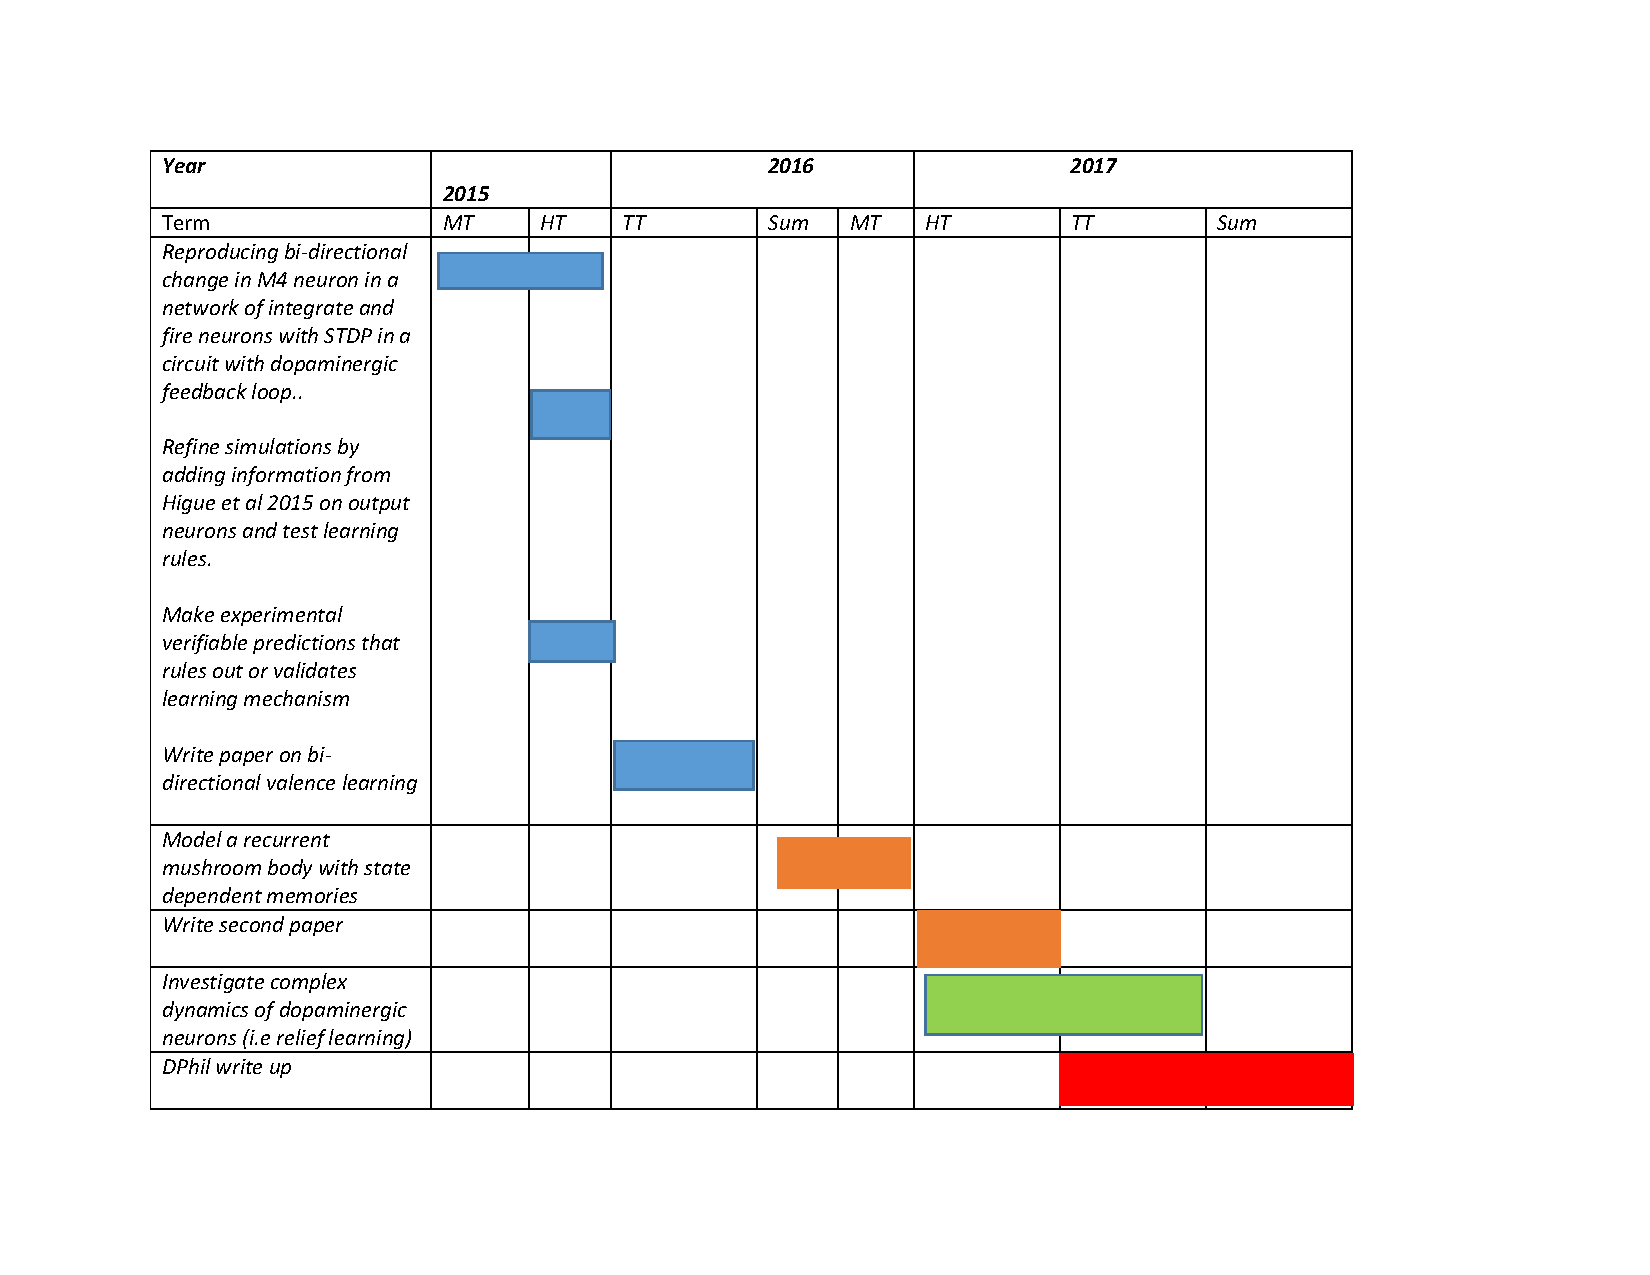
\includegraphics[scale=0.7]{chapter1/Timeline}\selectlanguage{english}%
\end{figure}
\selectlanguage{english}%

